%EP 2 de Laboratório de Simulação e Computação
%Aluno: Daniel Oliveira Caires
%Numero USP: 5197211
%Curso: Bacharelado em Matemática Aplicada e Computacional
%Turma 54 - Período Noturno

\documentclass[a4paper,12pt]{article} 
\usepackage[brazil]{babel}
\usepackage[utf8]{inputenc} 
\usepackage{amsmath}
\usepackage{amssymb}
\usepackage{graphicx}

\title{Laboratorio de Simulação e Computação - Relatório do Trabalho 2}
\author{Daniel Caires}
\date{}

\begin{document}
\maketitle
	\section{Sistema}
		\paragraph{Linguagem:} python com biblioteca numpy
		\paragraph{Como utilizar:} O programa não requer nenhum tipo de entrada de dados. Basta rodar o script utilizando o python
		\paragraph{Saída:} o programa imprime no terminal a média da medida de dispersão escolhida para cada valor de $n$ solicitado no enunciado do problema.

	\section{O problema}
		No quadrado $[0,1]\times[0,1]$ sorteie $n$ pontos $(x,y)$ aleatórios. \\
		Divida o quadrado em 100 ladrilhos de áreas iguais e contabilize o número de pontos sorteados em cada ladrilho. Calcule uma medida de dispersão para o número de pontos por ladrilho.\\ %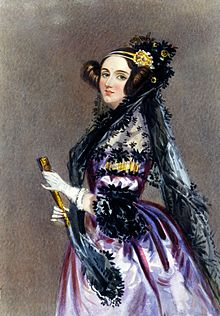
\includegraphics[scale=0.5]{ada.jpg}
		Repita o experimento 100 vezes e calcule a média dos valores encontrados para a medida de dispersão escolhida.\\
		O procedimento deve ser feito para $n=\{2^5,2^{10},2^{15},2^{20}\}$\\
		\paragraph{Questão 1:} Qual é a medida de dispersão adequada?\\
		\paragraph{Questão 2:} Mostre que a medida de dispersão escolhida decai conforme $n$ aumenta.

	\section{Solução}
		Para gerar os pontos aleatórios, foi utilizada a função random.rand() da biblioteca numpy do python.\\
		Essa função gera números pseudo-aleatórios entre 0 e 1. Uma vez que o par de númeromeros aleatórios $(x,y)$ foi gerado, determinamos o ladrilho correspondente, simplesmente multiplicando o número aleatório encontrado por 10 e pegando apenas a parte inteira. Feito isso, incrementamos um ponto ao ladrilho correspondente numa matriz de ladrilhos.\\
		Ao final do experimento contabilizamos o número de pontos em cada ladrihlo e calculamos a medida de dispersão.
		\paragraph{Questão 1:} A medida de dispersão escolhida foi o coeficiente de variação. Como nosso objetivo é comparar o comportamento da dispersão conforme o número de pontos cresce, essa medida é a mais adequada, pois para diferentesnúmeros de pontos, a ordem de grandeza da quantidade de pontos por ladrilho varia. Sendo assim, é adequado usarmos uma medida de dispersão ponderada pela média dos dados, no nosso caso, escolhemos o coeficiente de variação, também chamado de desvio padrão relativo, corresponde ao desvio padrão, dividido pela média.
		\paragraph{Questão 2:} O aumento no número de pontos representa um decréscimo significante no coeficiente de variação, como mostra a tabela abaixo que corresponde à saída de uma execução do programa:\\
		\begin{tabular}{c | c}
			n & Coeficiente de variação\\
			\hline
			$2^5$  & 1,76953092294\\			
			$2^10$ & 0,308209693849\\			
			$2^15$ & 0,0549925541159\\			
			$2^20$ & 0,00960329854126\\			
		\end{tabular}
		

\end{document}
